\chapter{着色}

\section{平方反比定律}

光线从光源到$r$位置光的强度满足平方反比定律
\begin{equation}
    Intensity=\frac{I}{r^2}
\end{equation}
\begin{figure}[H]
    \centering
    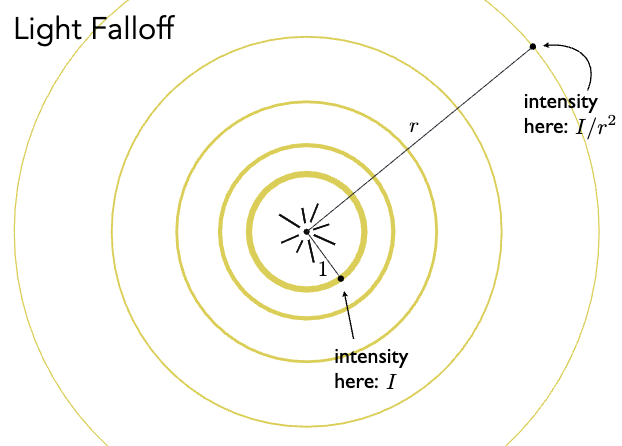
\includegraphics[scale=0.4]{figures/光强的平方反比定律.png}
    \caption[short]{光强的平方反比定律}
\end{figure}

光线经过反射被人眼观测,但是传播到$r$处的光并非所有能量都被人眼接收,由于接受光线的角度不一样,被物体吸收的光强也会衰减。

\begin{figure}[H]
    \centering
    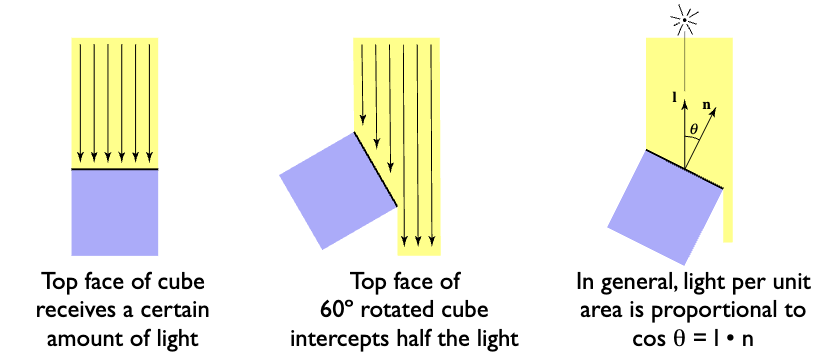
\includegraphics[scale=0.4]{figures/光强衰减.png}
    \caption[short]{光强的吸收}
\end{figure}

\section{Blin-Phong 反射模型}

Blin-Phong 反射模型描述了由\textsl{漫反射(Diffuse)}、\textsl{镜面反射(Specular)}、\textsl{环境光反射(Ambient)}组成。主要的表述形式如下
\begin{equation}
    \begin{aligned}
          L&=L_a+L_d+L_s\\
          &=k_aI_a+k_d(I/r^2)max(0,\mathbf{n}\cdot \mathbf{l})+k_s(I/r^2)max(0,\mathbf{n}\cdot \mathbf{h})^p
    \end{aligned}
\end{equation}

\begin{figure}[H]
    \centering
    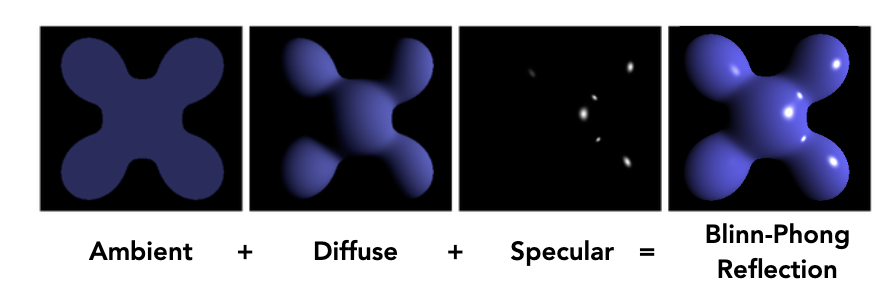
\includegraphics[scale=0.45]{figures/反射模型.png}
    \caption[short]{Blin-Phong 反射模型}
\end{figure}

我们下面分别解释每一项的意思,假设$I$是入射光的单位向量,$n$是平面法向量,$v$是观测方向的向量,
$k_d$系数在Blinn-Phong光照模型中是描述材质表面对漫反射光的吸收程度的参数,它影响了表面在漫反射光照下的亮度和颜色
$k_s$通常与光源的位置、观察者的位置以及材质的光泽程度等因素相结合,用来计算镜面反射光的强度。增加$k_s$的值会使得材质表面的镜面反射更加明显,反之则会减弱镜面反射的效果。
$k_a$是Blinn-Phong光照模型中的环境光系数,用于描述材质表面对环境光的反射程度。环境光是场景中所有光源的综合效果,它无处不在,没有特定的入射方向,而是均匀地照亮了整个场景。环境光系数ka表示了材质表面对环境光的反射程度。

\subsection*{漫反射$L_d$}

\begin{figure}[H]
    \centering
    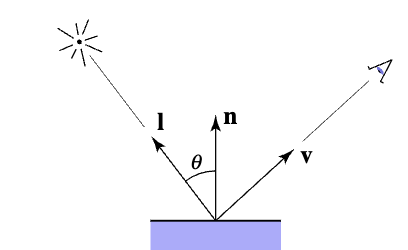
\includegraphics[scale=0.45]{figures/漫反射.png}
    \caption[short]{反射模型}
\end{figure}

当光线垂直射向物体表面,接收到的光线亮度或者强度是100,当光线和物体表面成角60度时,原来的六根光线只有三根光线被接收到,原因是因为物体表面的法线向量和入射方向的夹角为60
,$cos60\times6$就是三根光线。因此,接收到的光线的亮度或者强度与入射光线与平面法线的夹角有关,。
所以接收到的光照强度为
\begin{equation}
    (I/r^2)max(0,\mathbf{n}\cdot \mathbf{l})
\end{equation}


$L_d$是漫反射的光强,$I/r^2max(0,\mathbf{n}\cdot \mathbf{l})$为到达\textsl{着色点(shading point)}的光照能量,$k_d$是物体吸收光照的系数,

\subsection*{镜面反射}

镜面反射就是\textsl{高光},光线经过完全反射的向量和观测者方向向量存在一定的角度,如下图所示

\begin{figure}[H]
    \centering
    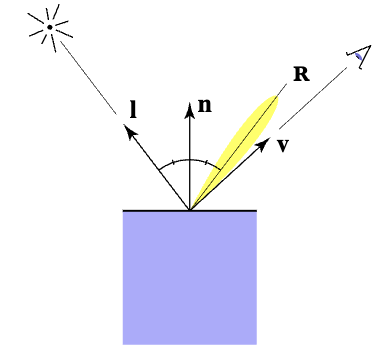
\includegraphics[scale=0.45]{figures/高光.png}
    \caption[short]{高光}
\end{figure}

根据入射光线和法线向量,可以得到反射光想的方向,根据反射光线的方向与视角方向的夹角计算人眼接收到光线的强度,这种高光模型称为\textsl{phong模型}

Blinn-Phong对该模型进行了改进,根据光线方向和视角方向引入了\textsl{半程向量},如下图所示,半程向量与法线向量的夹角的cos就间接表示了视角和反射光线的夹角的cos

\begin{figure}[H]
    \centering
    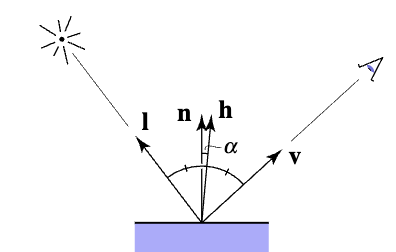
\includegraphics[scale=0.45]{figures/半程向量.png}
    \caption[short]{半程向量}
\end{figure}

所谓\textsl{半程向量}定义如下

\begin{equation}
    \begin{aligned}
        h = \frac{\mathbf{v}+\mathbf{l}}{\Vert\mathbf{v}+\mathbf{l}\Vert}
    \end{aligned}
\end{equation}

直观理解就是$\mathbf{l}$向$\mathbf{v}$方向旋转夹角的一半后进行归一化得到的向量。这时$\mathbf{n}$
和$\mathbf{h}$的夹角等于$R$和$\mathbf{v}$的夹角。

所以镜面反射的光强可以表示为
\begin{equation}
    \begin{aligned}
        L_s &= k_s(I/r^2)max(0,cos\alpha)^p\\
            &= k_s(I/r^2)max(0,\mathbf{n}\cdot \mathbf{h})^p
    \end{aligned}
\end{equation}

为什么要加上一个指数$p$呢?之所以要加一个指数项,也是为了符合人们的直觉,可以这样想
,比如当我们用镜子去晃别人的眼睛,镜子稍微偏转几度,就可能让被晃的人感觉光线强度变化很大,所
以,加了一个指数,就是让角度稍微一变化,光线强度就会由剧烈的波动,cos的指数函数图如下

\begin{figure}[H]
    \centering
    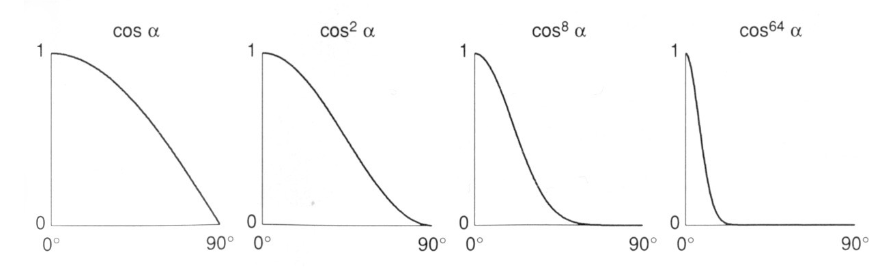
\includegraphics[scale=0.5]{figures/镜面反射幂的意义.png}
    \caption[short]{镜面反射幂的意义}
\end{figure}

\subsection*{环境光反射}

由与环境光和入射光和观测方向都没关系,因此只需乘一个常数$k_a$
\begin{figure}[H]
    \centering
    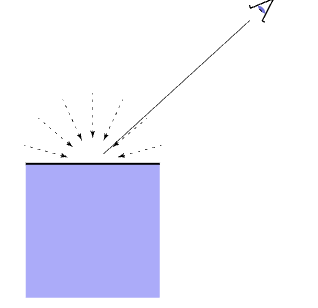
\includegraphics[scale=0.5]{figures/环境光反射.png}
    \caption[short]{环境光反射}
\end{figure}

\section{着色频率}

通过光照模型可知,最终的光照结果和光照点的法线向量关系很大。所以,根据不同的法线向量,就有不同的着色方法。在图形学中,法线分为:\textsl{面法线、顶点法线}和\textsl{像素法线}。光照和这三种法线相互作用,就有了三种不同的渲染频率。

\subsection*{面着色(Flat shading)}

面着色就是利用物体面表上的每个三角形的法线向量进行光照强度的计算,进而决定物体表面的颜色。该方法效果较差(物体表面不光滑,棱角较多)
\begin{figure}[H]
    \centering
    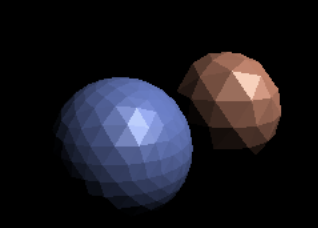
\includegraphics[scale=0.6]{figures/面着色.png}
    \caption[short]{面着色}
\end{figure}
\subsection*{顶点着色(Gouraud shading)}

顶点着色就是利用每个顶点的法向量来计算光照强度,得到三个顶点的颜色后,通过插值的方式来对面内的点的像素进行计算
\begin{figure}[H]
    \centering
    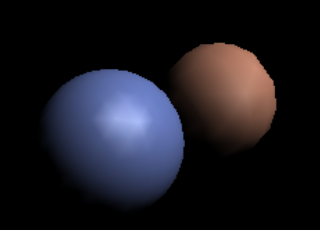
\includegraphics[scale=0.6]{figures/顶点着色.png}
    \caption[short]{顶点着色}
\end{figure}

首先如何计算每个顶点的法线向量?方法就是将所有共享该顶点的三角形面的法线向量计算出来,之后,将这些法线向量相加求平均,如下图所示
\begin{figure}[H]
    \centering
    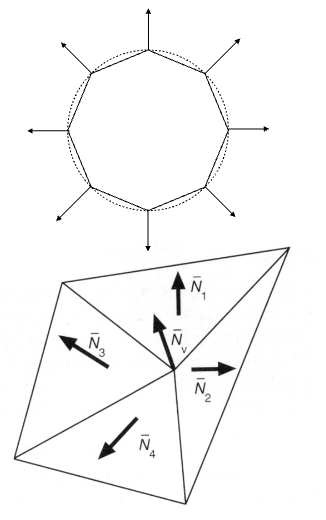
\includegraphics[scale=0.5]{figures/顶点法向量.png}
    \caption[short]{顶点法线}
\end{figure}

\begin{equation}
    N_v=\frac{\sum_iN_i}{\Vert\sum_iN_i\Vert}
\end{equation}

这样,就能得到每个顶点的法线向量,继而根据光照模型就能算出每个顶点的像素,

\subsection*{插值}

假设经过光照模型,已经得到了顶点的像素,我们通过插值的方法补充顶点之间像素。两个顶点之间直线的插值
\begin{equation}
    p=(1-t)a+tb
\end{equation}

只要把$a,b$两点的顶点像素数据代入,通过调节$t$的变化,便能生成一条线的像素数据。

对于三角形,如何进行插值呢?

\begin{figure}[H]
    \centering
    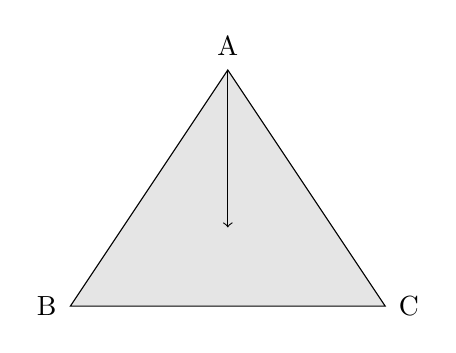
\begin{tikzpicture}
        \node (a) at (-0.3,0) {B};
        \node (a) at (2,3.3) {A};
        \node (a) at (4.3,0) {C};
        \node (b) at (1,0.7) {P};
        \filldraw[fill=gray!20!white, draw=black] (0,0) -- (4,0) -- (2,3) -- cycle;
        \draw [->] (2,3) -- (2,1) ;
    \end{tikzpicture}
    \caption[short]{三角形}
\end{figure}

对于三角形$\triangle ABC$内部任意一个点$P$,由于三角形是一个$2-$单形,必然存在$\alpha$、$\beta$
\begin{eqnarray}
    \overrightarrow{AP}=\alpha \overrightarrow{AB}+\beta \overrightarrow{AC}
\end{eqnarray}

展开有

\begin{equation}
    P-A=\alpha(B-A)+\beta(C-A)
\end{equation}

设$\gamma=1-\alpha-\beta$整理得到

\begin{equation}
    P=\gamma A+\alpha B+\beta C
\end{equation}

\subsection*{像素着色(Phong shading)}

像素着色是着色频率最高的方式,直接对每个像素点进行着色。

